\chapter{Catching Attackers in Restricted Network Zones}
\label{chap:concept}

Our T-Pot identified a flood of threads when it was widely available on the Internet.
However, capacious networks do have separated compartments and usually services are not directly available without any protection.
Zoning is a well-known method to segment a network.
Heidelberg University applies zoning, and thus, it is an interesting question if any attacker probes services outside or within the network.
To detect any dubious packets in the network we present a concept using a honeypot-like detection tool.
We show that attacks in a restricted network zone of the Heidelberg University's internal network occur, and contributed to an adaption of the stateless firewall.
Thus, improving the security of the network.

\section{University Network}

Honeypots that are accessible via the Internet do receive a broad range of attacks.
As \citet{Spitzner2003} noted, a honeypot is not strictly bound to run in a \ac{dmz} or in a network with direct Internet access.
The correct location has to be chosen based on the goals of the honeypot.
For example, one goal could be to catch attackers behind a perimeter firewall to reveal leaks or vulnerabilities.
Beforehand, our honeypot was broadly available on the Internet, and attackers could probe it easily.
It collected on average $\numprint{55000}$ attacks per day, resulting in a total amount of $\numprint{786564}$ attacks.
Zoning a network into logical groups mitigates the risk of an open network.
Thus, our T-Pot would receive significantly fewer attacks in a controlled network zone.
A network infrastructure is segmented into the same communication security policies and security requirements.
For example, the Canadian government created their own baseline for infrastructures, called Baseline Security Architecture Requirements for Network Security Zones in the Government of Canada (ITSG-22).
The four most common zones are:
\begin{enumerate*}[label=(\roman*)]
    \item Public Zone (PZ) which is entirely open,
    \item Public Access Zone (PAZ) which interacts as an interface between the PZ and internal services,
    \item Operations Zone (OZ) which processes sensitive information, and
    \item Restricted Zone (RZ) including business critical services
\end{enumerate*}.
A network zone restricts access and controls data communication flows. \cite{csec2021}

\begin{figure}[ht]
    \centering
    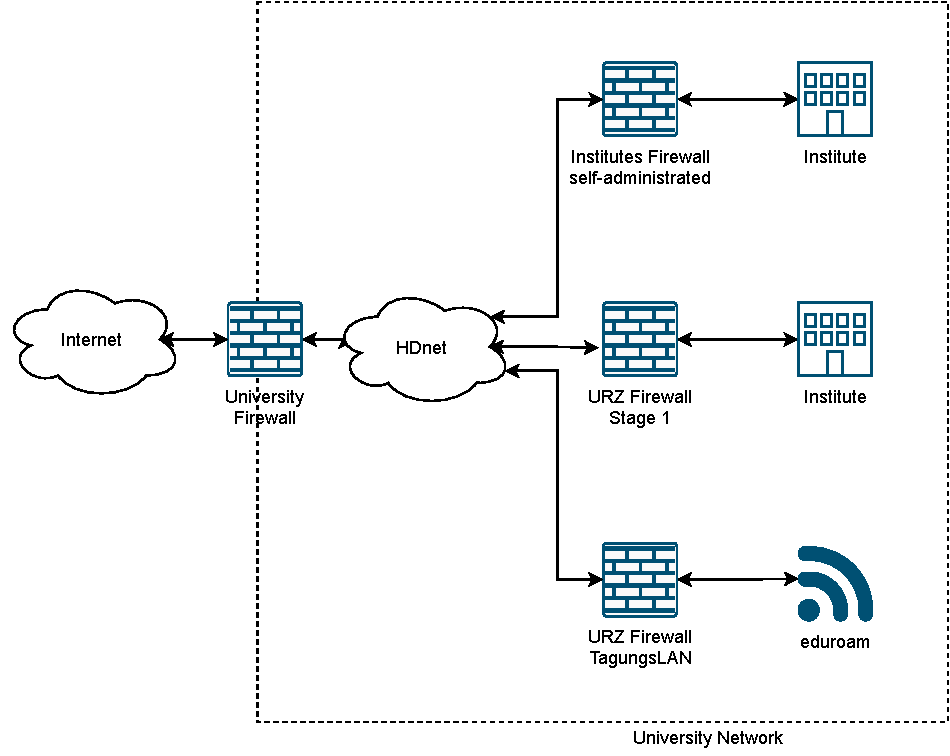
\includegraphics[width=\textwidth]{figures/university-network.pdf}
    \caption[Draft of the University network]{Draft of the University network. The URZ firewall represents the stateful firewall. The \enquote{TagungsLAN} i}
    \label{fig:university-network}
\end{figure}

The network at the Heidelberg University includes a central stateless firewall (\ac{acl}) that enfolds all institutes.
It entails a default blacklist that blocks certain services such as SMTP, NCP, or SNMP, and a stateless filter provided by BelWÜ.
Inside the network, each institute has the possible to either use a pre-defined stateless firewall provided by the University Computing Center Heidelberg, or use a self-administrated firewall.
\autoref{fig:university-network} outlines the association between these components.
The internal \enquote{HDnet} enables the communication between institutes without leaving the internal network.
Institute firewalls can be set up by each institute and is self-administrated.
They do have the possibility to use \ac{soho} routers\footnote{\ac{soho} router is a broadband router used in small offices and home offices environments.} to disconnect certain network zones from the network.
It is recommended to configure the global \ac{acl} as a fall back solution in case of any downtime.
The University Computing Center Heidelberg offers stateless firewall for router interfaces or VLANs.
This stateful firewall whitelists certain services and splits up into four stages.
Each stage can be individually activated per router interface.
Its key value is to maintain a baseline security to avoid any misconfigurations and port scans.
\autoref{tab:overview-security-zone} outlines these stages including the IP address range.
Before applying one of these zones, the respective network has to oblige to client IP addresses below \ipAddress{129.206.218.240/24}.
In addition, \ipAddress{129.206.218.1} is allocated for the gateway.
A network has to adhere to these obligations if it applies any of these pre-defined stages.

\begin{table}
    \centering
    \caption[Overview of firewall stages]{
        Overview of firewall stages at the University Heidelberg.
        As an example we applied the rules to subnet \ipAddress{129.206.218.0/24}.
        Any rule does apply to any another subnet.
    }
    \begin{tabularx}{\linewidth}{l|XX}
        \toprule
        \textsc{Name} & \textsc{Description}                      & \textsc{range}                     \\
        \hline
        Stage 0       & Filters broadcast communication           & \ipAddress{129.206.218.0-15/24}    \\
                      & No filtering                              & \ipAddress{129.206.239.16-255/24}  \\
        \hline
        Stage 1       & Allows common network protocol            & \ipAddress{129.206.239.0-255/24}   \\
                      & Allows services                           & \ipAddress{129.206.239.240-255/24} \\
        \hline
        Stage 3       & Internet access only via internal proxies & \ipAddress{129.206.239.0-255/24}   \\
        \hline
        Stage 4       & Only internal network communication       & \ipAddress{129.206.239.0-255/24}   \\
        \bottomrule
    \end{tabularx}
    \label{tab:overview-security-zone}
\end{table}

An interesting question is if attackers have access to restricted zones at the Heidelberg University.
It arises during the research of T-Pot if an adversary would try to probe any hosts in the internal University network.
In order to detect such events we present honeypot-like packet detection application that helps to identify any threats in a network.
In addition, it offers to deploy multiple instance and collect their data in a centralized instance.

\section{Honeypot-like Connection Detection Tool}

Recording and investigating connection attempts assimilates new honeypots.
Respectively, we will present a new honeypot-like detection tool called MADCAT.
It has been developed by the BSI, and helps us to log any connection attempt being made on our host machine.
The acronym MADCAT stands for Mass Attack Detection Connection Acceptance Tools.
It works as a honeypot-like detection application with low interaction level.
Its key idea is to log every connection attempt and further process it to retrieve credentials, or shell exploitation.
\autoref{fig:madcat-architecture} gives an inside how MADCAT works.
It runs on an Ubuntu distribution either $18.04$ or $20.04$.
We have tested it on Ubuntu $18.04$.
It processes packets from any interface that has been configured.
As an example, we could process Ethernet and wireless packets.
MADCAT itself consists of six independent modules for TCP, UDP, ICMP, and RAW packets that communicating with each other through a pipeline.
A module is responsible for analyzing packets and logging the results in a queue.
In addition, UDP and TCP offers a proxy to tunnel packets to another service.
TCP postprocessor reads every 5 seconds the newly arrived TCP packets and processes them accordingly.
It resolves packets to log data including source IP address, protocol and event type.
The enrichment processor is the final process step.
Its purpose is to log all written packets of the queue in a specified format for further analyzation.
The key idea of MADCAT is to get an inside if attackers have access to a certain network.
In contrast to T-Pot, we do not want to know what specific attacks are operated on our honeypot.
Instead, we do want to ensure that no one else than authorized users have access.
Especially in high confidential areas, no attacker should be capable of sending even a single packet to a host in the network.
Tracking packets on a detailed level is not provided by the vast range of honeypots.

% TODO: Conecpt ueberarbeiten, beheben der Darstellung
\begin{figure}
    \centering
    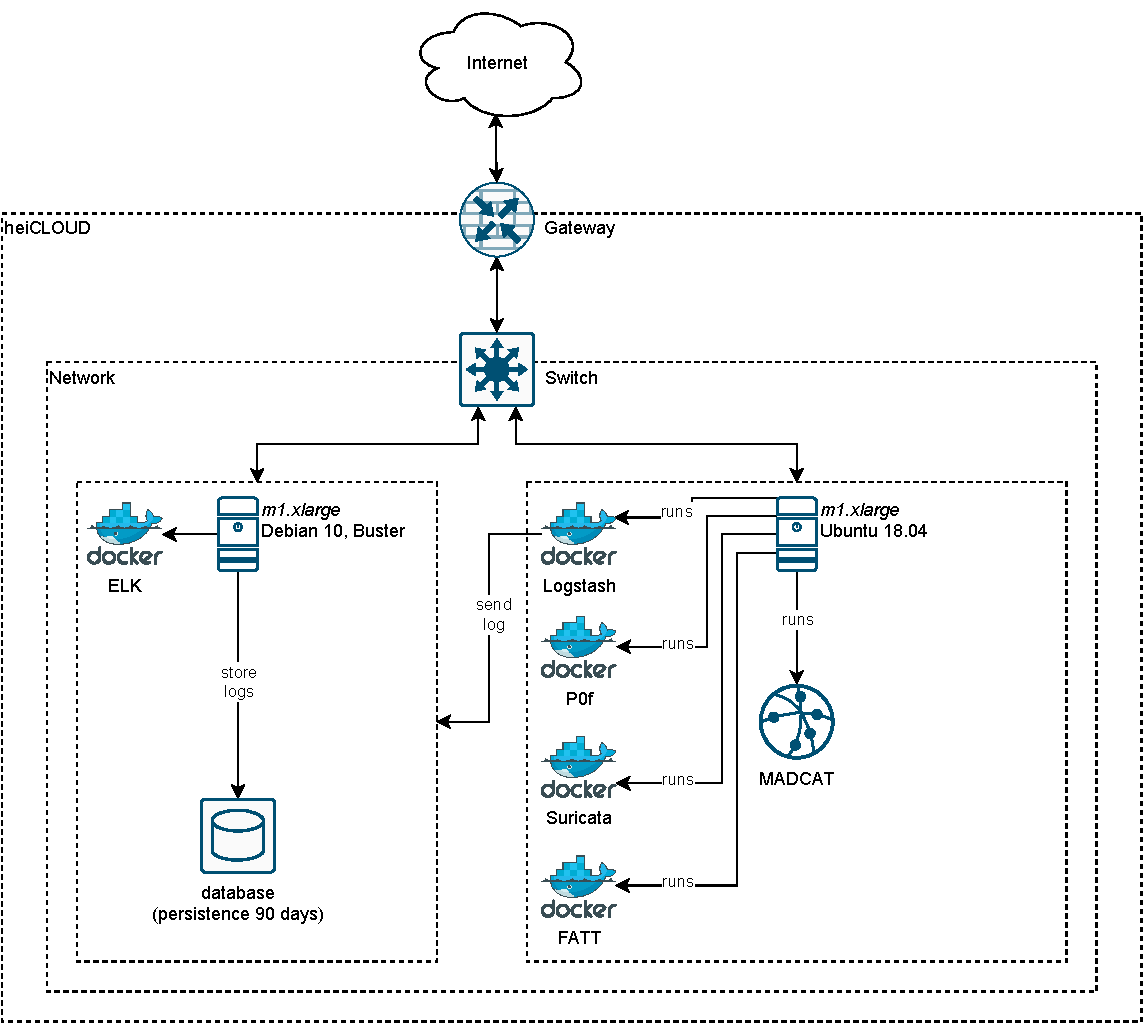
\includegraphics[width=\textwidth]{figures/heicat-conecpt.pdf}
    \caption[Concept to detect connection attempts]{Concept to detect connection attempts. Kibana and Elasticsearch are deployed in heiCLOUD.}
    \label{fig:heicat-concept}
\end{figure}

In addition, we will deploy a T-Pot instance to have comparison data to our new concept.
We focus on the \ipAddress{129.206.218.0/24} and \ipAddress{147.142.0.0/16} subnet.
The \ipAddress{129.206.218.0/24} subnet is used within University Computing Center Heidelberg building.
Every client in the building has a compelling connection in this subnet.
Otherwise, an Internet connection would not be feasible.
The subnet \ipAddress{147.142.0.0/16} connects clients to \enquote{eduroam}\footnote{The eduroam is an international Wi-Fi internet access point for researchers.}.
Like the four stages of the institute firewall, the \enquote{eduroam} network, also called \enquote{Tagungslan}, builds various permits into the subnet.
One essential important % TODO: Example
Our instances are located in the building with IP addresses \ipAddress{129.206.219.65} and \ipAddress{129.206.219.88}.
\autoref{fig:heicat-concept} outlines our concept using MADCAT and a separate instance to visualize our data.
The first instance with IP address \ipAddress{129.206.5.157} provides Kibana, and Elasticsearch to visualize and crawl logs.
The honeypot with IP address \ipAddress{129.206.5.88} consists of MADCAT in conjunction with P0f, Suricata, and FATT.
Like T-Pot, we use Logstash to forward our data to Elasticsearch.
One benefit is the centralized approach to store data.
This allows to randomly deploy more instances to collect data from other zones.

\begin{figure}
    \centering
    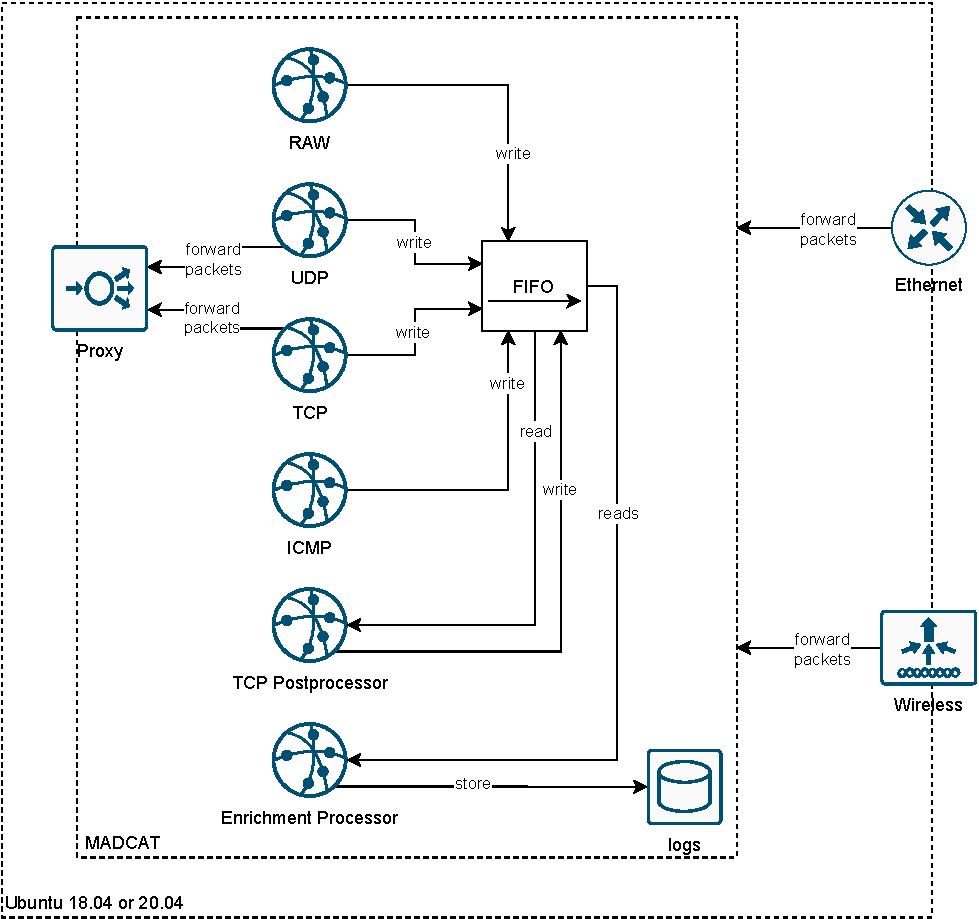
\includegraphics[width=\textwidth]{figures/heicat-architecture.pdf}
    \caption[Visualization of the MADCAT packet flow]{Visualization of the MADCAT packet flow starting at the network interface. The Ethernet and wireless interface forwards packets to the desired module.}
    \label{fig:madcat-architecture}
\end{figure}

\section{Results} % TODO: Mehr Ergebnisse, Attacken zeigen, Grafiken

Our MADCAT and T-Pot has been deployed for three weeks.
In total, MADCAT received \numprint{35372} packets.
Overall, flow ($66.62\%$) and RAW ($33.26\%$) packets.
Syn packets with a 
T-Pot 
\autoref{fig:madcat-protocols} shows the protocol distribution.

\autoref{fig:madcat-attack-distribution} shows the attack distribution indicating the origin of an IP address.
Most of the connection attempts are originated from the United States, Germany, and China.
As we have shown beforehand in \autoref{chap:cloud-security}, geographical information only outlines the last know location of a node.
Like our results in heiCLOUD, we assume that this information is not reliable as an indicator.
Nevertheless, it is an interesting to see 

% TODO: Bessere Caption
\begin{figure}[ht]
    \centering
    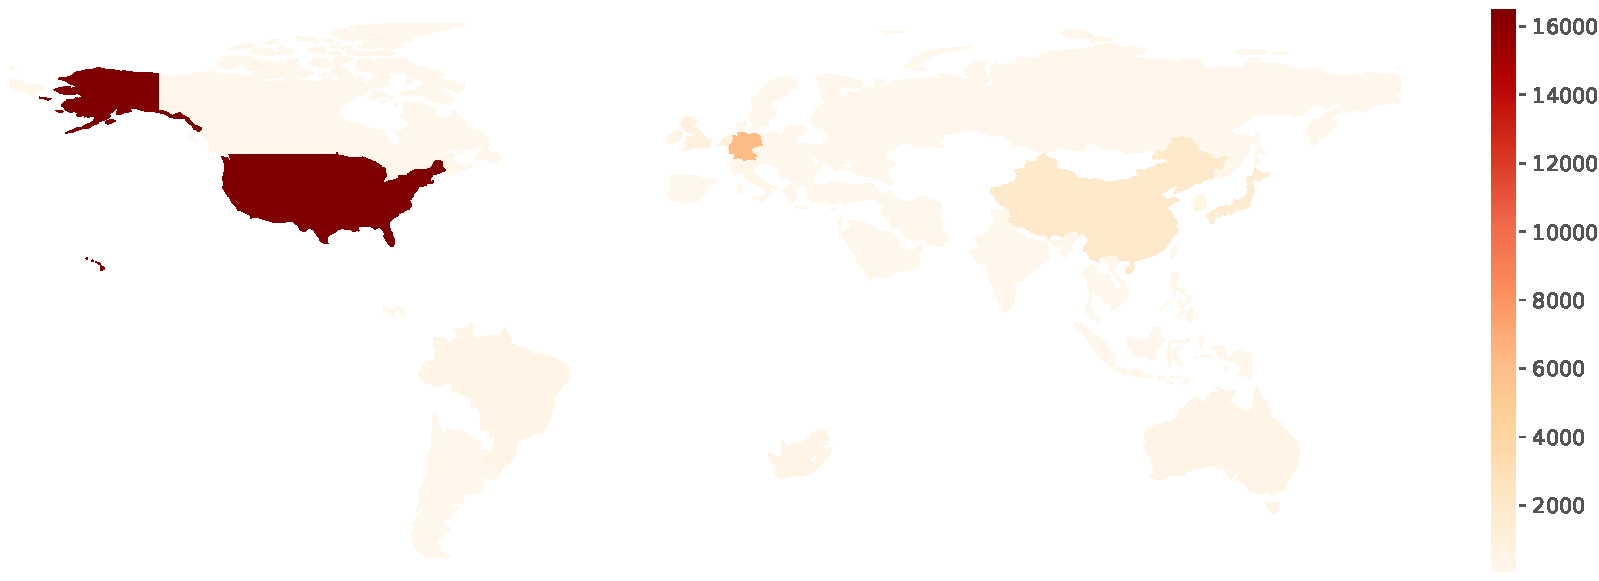
\includegraphics[width=\textwidth]{figures/madcat-overview-map.pdf}
    \caption[Attack distribution of MADCAT]{Attack distribution of MADCAT. USA, Russia, China, and Germany are the most attacking countries. Timestamp; 22nd of September to 22nd of November.}
    \label{fig:madcat-attack-distribution}
\end{figure}

% TODO: Bessere Caption
\begin{figure}[ht]
    \centering
    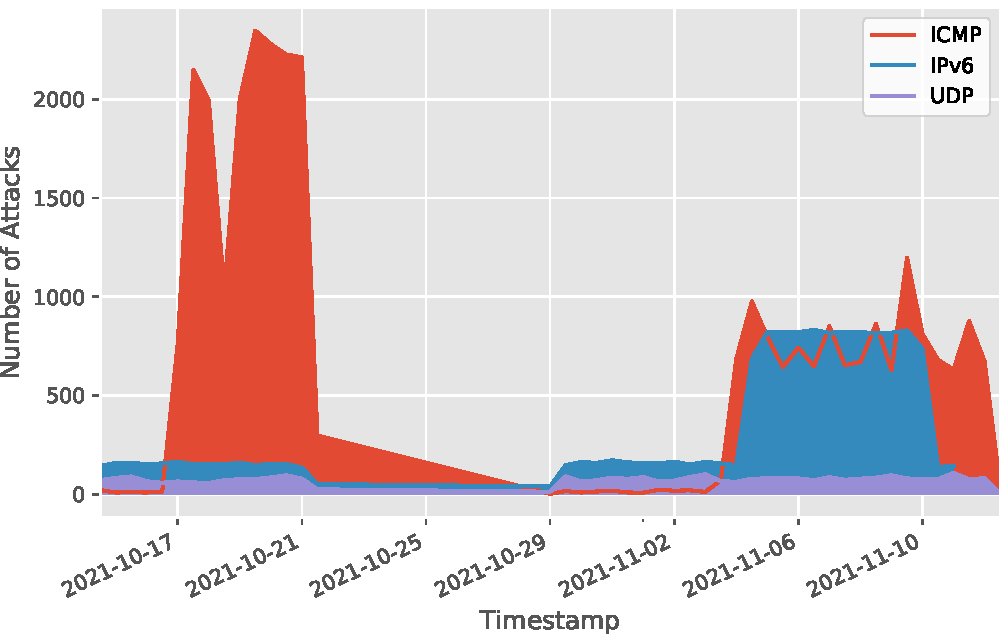
\includegraphics[width=\textwidth]{figures/madcat-protocol-usage.pdf}
    \caption[Protocol distribution of MADCAT]{Protocol distribution of MADCAT. ICMP, IPv6 and UDP are the most used protocols. Timestamp; 22nd of September to 22nd of November.}
    \label{fig:madcat-protocols}
\end{figure}

Suricata identified odd behaviors in the network.

Crawling through our packets, we identified a few exploitation attempts.
SIP and SMB are allocating the fast majority of 

\begin{figure}
    \lstinputlisting[language=bash, caption={MADCAT connection attempt to exploit SIP connection}, label={lst:sip-exploitation}]{listings/exploit-sip.txt}
\end{figure}

\begin{figure}
    \lstinputlisting[language=bash, caption={MADCAT connection attempt to exploit SMB connection}, label={lst:smb-exploitation}]{listings/exploit-smb.txt}
\end{figure}

% TODO: Add discussion
